\documentclass[11pt,a4paper,oneside, titlepage,reqno]{amsproc}
\usepackage{changepage}
\usepackage{mathtext} % русские буквы в формулах
\usepackage[T2A]{fontenc}
\usepackage[utf8x]{inputenc}
\usepackage{ucs}
\usepackage{cmap}
\usepackage[english,russian]{babel}
\usepackage{graphicx}
%\usepackage{concrete}
%\usepackage{amsmath}
%\usepackage{amsfonts}
\usepackage{amssymb}
\usepackage{dcolumn}
\usepackage{booktabs}
\usepackage{ctable}
\usepackage{multirow}

\newcommand{\specialcell}[2][c]{%
  \begin{tabular}[#1]{@{}c@{}}#2\end{tabular}}
\oddsidemargin = 0pt
\textwidth = 14 cm
\topmargin = -2 cm
\textheight = 24 cm
\makeatletter
\renewcommand{\theequation}{\thesection.\arabic{equation}}
\@addtoreset{equation}{section}
\newcommand{\eq}{\begin{equation}}
\newcommand{\eeq}{\end{equation}}
\newcommand{\fr}{\frac}
\newcommand{\mf}{\mathfrak}
\newcommand{\sub}{\subsection}
\newcommand{\subsub}{\subsubsection}
\newcommand{\definition}{\theoremstyle{definition}}
\newcommand{\mult}[2]{\genfrac{\left[}{\right.}{0pt}{}{#1}{#2}}
\renewcommand{\qed}{\begin{center} $\mathsf{QED}$ \end{center}}
\newcommand{\al}{\alpha}
\newcommand{\comment}[1]{\marginpar{\Small{{\sl #1}}} }
\newcommand{\epigraph}[2]{\begin{flushright} {\em #1}\\#2\\[20 pt]
\end{flushright}}
\newcommand{\fx}[1]{\ensuremath{\mathit{f}_{#1}(x)}}
\newcommand{\re}[1]{(\ref{#1})}
\newcommand{\mh}{\mathit}
\newcommand{\itm}[1]{\begin{itemize}	\item #1 \end{itemize}}
\newcommand{\note}[1]{\begin{flushleft}\hbox{%
\vrule\hspace{.5em}\parbox{ .9\textwidth}%
{ #1}} \end{flushleft}}
\newcommand{\Al}{\ensuremath{\mathcal{A}}}
\newcommand{\@dotsep}{3.9}
\newcommand{\system}[1]{\eq\left\{ \begin{aligned} #1
\end{aligned}\right.\\[5 pt]\eeq}
\renewcommand{\phi}{\varphi}

% http://www.texnik.de/floats/caption.phtml
% This does spacing around caption.
%\setlength{\abovecaptionskip}{6pt}   % 0.5cm as an example
%\setlength{\belowcaptionskip}{9pt}   % 0.5cm as an example

%%%%%%%%%%%%%%%%%%%%%%%%%%%%%%%%%%%%%%%%%%%%%%%%%%%%%%%%%%%%%%%%%%%%%%%

\author{Соколовский Роман}
\begin{document}
\begin{titlepage}
\begin{center}
% Upper part of the page
\textsc{\LARGE ГУАП}\\[2cm]
\textsc{\LARGE Кафедра антенн и эксплуатации радиоэлектронной 
 аппаратуры}
\\[1cm]


 \begin{flushleft} \large
  \emph{Отчёт} \\
   \emph{защищен с оценкой}
   \\[0.5cm]
   \emph{Преподаватель}\\[-4mm]
   \HRule
\end{flushleft}
\begin{flushright}
Должность, уч. степень, звание \ \ \ \ \ \ \ подпись, дата \ \ \ \ \ \ \ инициалы, фамилия \\[10mm]
\end{flushright}

\textsc{\Large Отчёт о лабораторной работе №5:} \\[1cm]
\textsc{\Large ИССЛЕДОВАНИЕ ПОВЕРХНОСТЫХ ВОЛН, РАСПРОСТРАНЯЮЩИХСЯ ВДОЛЬ ПЛОСКИХ ЗАМЕДЛЯЮЩИХ СИСТЕМ.}\\[1.5cm]
% Title

% Author and supervisor

\begin{flushleft} \large
\emph{Работу выполнил:}\\
Студент\\ гр. 5025.\\[-4mm]
\HRule
\end{flushleft}
\begin{flushright}
подпись, дата \ \ \ \ \ \ \ инициалы, фамилия \\[10mm]
\end{flushright}

\vfill
% Bottom of the page
Санкт-Петербург, {\today}
\end{center}
\end{titlepage}

\section{Цель Работы}
\begin{itemize}
    \item Изучение законов отражения плоских электромагнитных волн от плоской проводящей
        поверхности
    \item Изучение структуры поля при нормальном и наклонном падении параллельно
        поляризованной волны на плоскую проводящую поверхность
    \item Изучение структуры поля при наклонном падении перпендикулярно поляризованной волны
        на плоскую проводящую поверхность
    \item Исследование распределения по нормали к экрану амплитуд составляющих электрического
        поля в зависимости от угла падения на проводящий экран параллельно поляризованной
        плоской электромагнитной волны
    \item Исследование волны, направляемой металлической границей раздела
    \item Исследование распределения амплитуж составляющих поля по нормали к экрану в
        зависимости от угла падения на проводящий экран параллельно и перпендикулярно
        поляризованных плоских электромагнитных волн.\\
\end{itemize}

\section{Схема Лабораторной Установки}
Схема лабораторной установки представлена на Рис. \ref{fig:scheme},
компонеты установки обозначены следующим образом:
\begin{enumerate}
    \item СВЧ-генератор
    \item излучающий пирамидальный рупор
    \item волновод прямоугольного сечения
    \item коаксиальный волновой переход
    \item полуволновой симметричный вибратор
    \item коаксиальный соединитель
    \item детекторная секция
    \item измерительный усилитель
    \item металлический стол с крестообразными прорезями
    \item плоский основной алюминиевый экран
    \item плоский дополнительный алюминиевый экран.
\end{enumerate}

\begin{figure}[h!]
    \begin{center}
        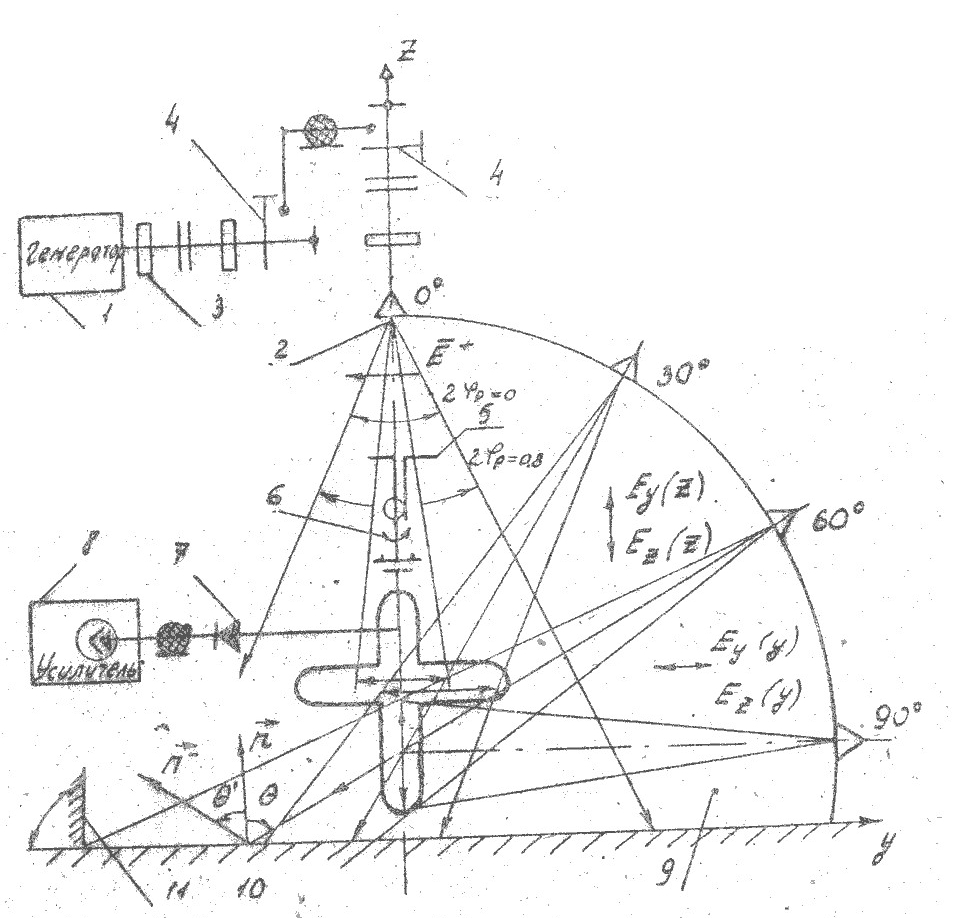
\includegraphics[width=0.60\textwidth]{scheme.jpg}
    \end{center}
    \vspace{-20pt}
    \caption{Принципиальная схема лабораторной установки}
    \label{fig:scheme}
\end{figure}

\newpage
\section{Результаты измерений и вычислений}
\subsection{Теоретические значения}
\subsubsection{$|\overline{E}_{\Sigma_{y,z}}(y,z)|$}
Суммарное поле можно записать в следующем виде:\\
\begin{equation}
    \left\{
    \begin{aligned}
        |\overline{E}_{\Sigma_y~norm}| &= 2\cos\theta\cdot\sin\beta_zz\\
        |\overline{E}_{\Sigma_z~norm}| &= 2\sin\theta\cdot\cos\beta_zz\\
    \end{aligned}
    \right.
    \label{eq:system}
\end{equation}

Из уравнения \ref{eq:system} видно, что узлы для составляющей суммарного поля модно вычислить
следующим образом:
\begin{equation}
    Z_{\max y} = Z_{\min zx} = (2p + 1)\frac{\Lambda z}{4},
\end{equation}
где
\subsubsection{$\Lambda_{yz}(\theta)$ теоретическое}
\begin{equation}
    \left\{
    \begin{aligned}
    \Lambda_z &= \frac{\lambda}{\cos\theta}\\
    \Lambda_y &= \frac{\lambda}{\sin\theta}\\
    \end{aligned}
    \right.
    \label{eq:lambdas}
\end{equation}

\subsection{Экспериментально вычисленные $\Lambda_{yz}(\theta)$}
На основе экспериментальных данных были получены следующие значения $\Lambda_{yz}$
\begin{equation}
    \left\{
    \begin{aligned}
        \Lambda_z(0^\circ) &= 36~\text{mm}\\
        \Lambda_z(30^\circ) &= 32~\text{mm}\\
        \Lambda_z(60^\circ) &= 72~\text{mm}\\
    \end{aligned}
    \right.
    ~ ~ ~ ~ 
    \left\{
    \begin{aligned}
        \Lambda_y(30^\circ) &= 52~\text{mm}\\
        \Lambda_y(60^\circ) &= 40~\text{mm}\\
    \end{aligned}
    \right.
    \label{eq:experimental}
\end{equation}
\vspace{6pt}

\subsection{Таблицы результатов измерений и вычислений}
Результаты экспериментального исследования составляющих параллельно поляризованной волны
приведены в таблицах 1 и 2.

\begin{centering}
\begin{table}[h!]
\newcolumntype{W}{D{.}{.}{2.3}}
\begin{adjustwidth}{-1cm}{}
\vspace{10pt}
\begin{tabular}{cccccccccc}
\toprule %[-2.08em]
\multicolumn{6}{c}{$|\overline{E}_{\Sigma_y}(z)|$} &
\multicolumn{4}{c}{$|\overline{E}_{\Sigma_z}(z)|$} \\[5 pt]
\multicolumn{2}{c}{$\theta = 0^\circ$} & 
\multicolumn{2}{c}{$\theta = 30^\circ$} & 
\multicolumn{2}{c}{$\theta = 60^\circ$} &
\multicolumn{2}{c}{$\theta = 30^\circ$} & 
\multicolumn{2}{c}{$\theta = 60^\circ$} \\
$z$,~mm & $\sqrt{\frac{\alpha}{\alpha_{\max}}}$ & 
$z$,~mm & $\sqrt{\frac{\alpha}{\alpha_{\max}}}$ & 
$z$,~mm & $\sqrt{\frac{\alpha}{\alpha_{\max}}}$ & 
$z$,~mm & $\sqrt{\frac{\alpha}{\alpha_{\max}}}$ & 
$z$,~mm & $\sqrt{\frac{\alpha}{\alpha_{\max}}}$ \\
 \midrule
20  &  0.415228  &  28  &  0.803219  &  14  &  0.395285  & 19  &  0.723747  &  46  &  0.748331  \\
22  &  0.473432  &  30  &  0.803219  &  16  &  0.395285  & 21  &  0.806718  &  48  &  0.83666   \\
24  &  0.776819  &  32  &  0.879883  &  18  &  0.395285  & 23  &  0.908514  &  50  &  0.894427  \\
26  &  0.946864  &  34  &  0.950382  &  20  &  0.467707  & 25  &  0.959497  &  52  &  0.959166  \\
28  &  1         &  36  &  0.983739  &  22  &  0.572822  & 27  &  0.992032  &  54  &  0.989949  \\
30  &  0.982607  &  38  &  1         &  24  &  0.684653  & 29  &  1         &  56  &  1         \\
32  &  0.890563  &  40  &  0.915811  &  26  &  0.790569  & 31  &  0.959497  &  58  &  1         \\
34  &  0.719195  &  42  &  0.861356  &  28  &  0.866025  & 33  &  0.899736  &  60  &  0.959166  \\
36  &  0.508548  &  44  &  0.803219  &  30  &  0.935414  & 35  &  0.835711  &  62  &  0.938083  \\
38  &  0.473432  &  -   &  -         &  32  &  0.976281  & 37  &  0.786796  &  64  &  0.883176  \\
-   &  -         &  -   &  -         &  34  &  1         & 39  &  0.776643  &  66  &  0.812404  \\
-   &  -         &  -   &  -         &  36  &  0.992157  & -   &  -         &  68  &  0.761577  \\
-   &  -         &  -   &  -         &  38  &  0.935414  & -   &  -         &  70  &  0.678233  \\
-   &  -         &  -   &  -         &  40  &  0.829156  & -   &  -         &  72  &  0.616441  \\
-   &  -         &  -   &  -         &  42  &  0.684653  & -   &  -         &  74  &  0.565685  \\
-   &  -         &  -   &  -         &  44  &  0.559017  & -   &  -         &  76  &  0.547723  \\
-   &  -         &  -   &  -         &  46  &  0.450694  & -   &  -         &  78  &  0.547723  \\
-   &  -         &  -   &  -         &  48  &  0.395285  & -   &  -         &  -   &  -         \\
-   &  -         &  -   &  -         &  50  &  0.353553  & -   &  -         &  -   &  -         \\
\bottomrule
\end{tabular}
\vspace{5 pt}
\caption{Зависимости составляющих $|\overline{E}_{\Sigma_y}(z)|$ и $|\overline{E}_{\Sigma_z}(z)|$} 
\end{adjustwidth}
\label{tab:tab1}
\end{table}
\end{centering}

\begin{centering}
\begin{table}[h!]
\newcolumntype{W}{D{.}{.}{2.3}}
%\begin{adjustwidth}{-1.5cm}{}
\vspace{10pt}
\begin{tabular}{cccccccc}
\toprule %[-2.08em]
\multicolumn{4}{c}{$|\overline{E}_{\Sigma_y}(y)|$} &
\multicolumn{4}{c}{$|\overline{E}_{\Sigma_z}(y)|$} \\[5 pt]
\multicolumn{2}{c}{$\theta = 30^\circ$} & 
\multicolumn{2}{c}{$\theta = 60^\circ$} &
\multicolumn{2}{c}{$\theta = 30^\circ$} & 
\multicolumn{2}{c}{$\theta = 60^\circ$} \\
$z$,~mm & $\sqrt{\frac{\alpha}{\alpha_{\max}}}$ &
$z$,~mm & $\sqrt{\frac{\alpha}{\alpha_{\max}}}$ &
$z$,~mm & $\sqrt{\frac{\alpha}{\alpha_{\max}}}$ &
$z$,~mm & $\sqrt{\frac{\alpha}{\alpha_{\max}}}$ \\
\midrule
14  &  0.62361   &  22  &  0.606977  &  34  &  0.680414  &  18  &  0.570088  \\
16  &  0.62361   &  24  &  0.675381  &  36  &  0.732828  &  20  &  0.591608  \\
18  &  0.65263   &  26  &  0.749269  &  38  &  0.816497  &  22  &  0.724569  \\
20  &  0.827759  &  28  &  0.858395  &  40  &  0.892354  &  24  &  0.758288  \\
22  &  0.922958  &  30  &  0.945905  &  42  &  0.952579  &  26  &  0.935414  \\
24  &  0.981307  &  32  &  1         &  44  &  0.981307  &  28  &  1         \\
26  &  1         &  34  &  0.955134  &  46  &  1         &  30  &  1         \\
28  &  0.981307  &  36  &  0.783604  &  48  &  0.981307  &  32  &  0.894427  \\
30  &  0.902671  &  38  &  0.648886  &  50  &  0.952579  &  34  &  0.758288  \\
32  &  0.816497  &  40  &  0.606977  &  52  &  0.892354  &  36  &  0.632456  \\
34  &  0.693888  &  -   &  -         &  54  &  0.805076  &  38  &  0.591608  \\
36  &  0.638284  &  -   &  -         &  56  &  0.745356  &  -   &  -         \\
38  &  0.62361   &  -   &  -         &  58  &  0.720083  &  -   &  -         \\
-   &  -         &  -   &  -         &  60  &  0.680414  &  -   &  -         \\
\bottomrule
\end{tabular}
\vspace{5 pt}
\caption{Зависимости составляющих $|\overline{E}_{\Sigma_y}(y)|$ и $|\overline{E}_{\Sigma_z}(y)|$} 
%\end{adjustwidth}
\label{tab:tab2}
\end{table}
\end{centering}

\subsection{Графики и рисунки}
Наиболее наглядным способом демонстрации и анализа структуры электромагнитного поля над
проводящей плоской поверхностью являются графики соответствующих зависимостей.
На рисунках \ref{fig:plot1}-\ref{fig:plot4} представлены графики различных составляющих
параллельно поляризованной волны, распространяющейся вдоль плоского проводящего экрана.

\begin{figure}[hb!]
    \begin{center}
        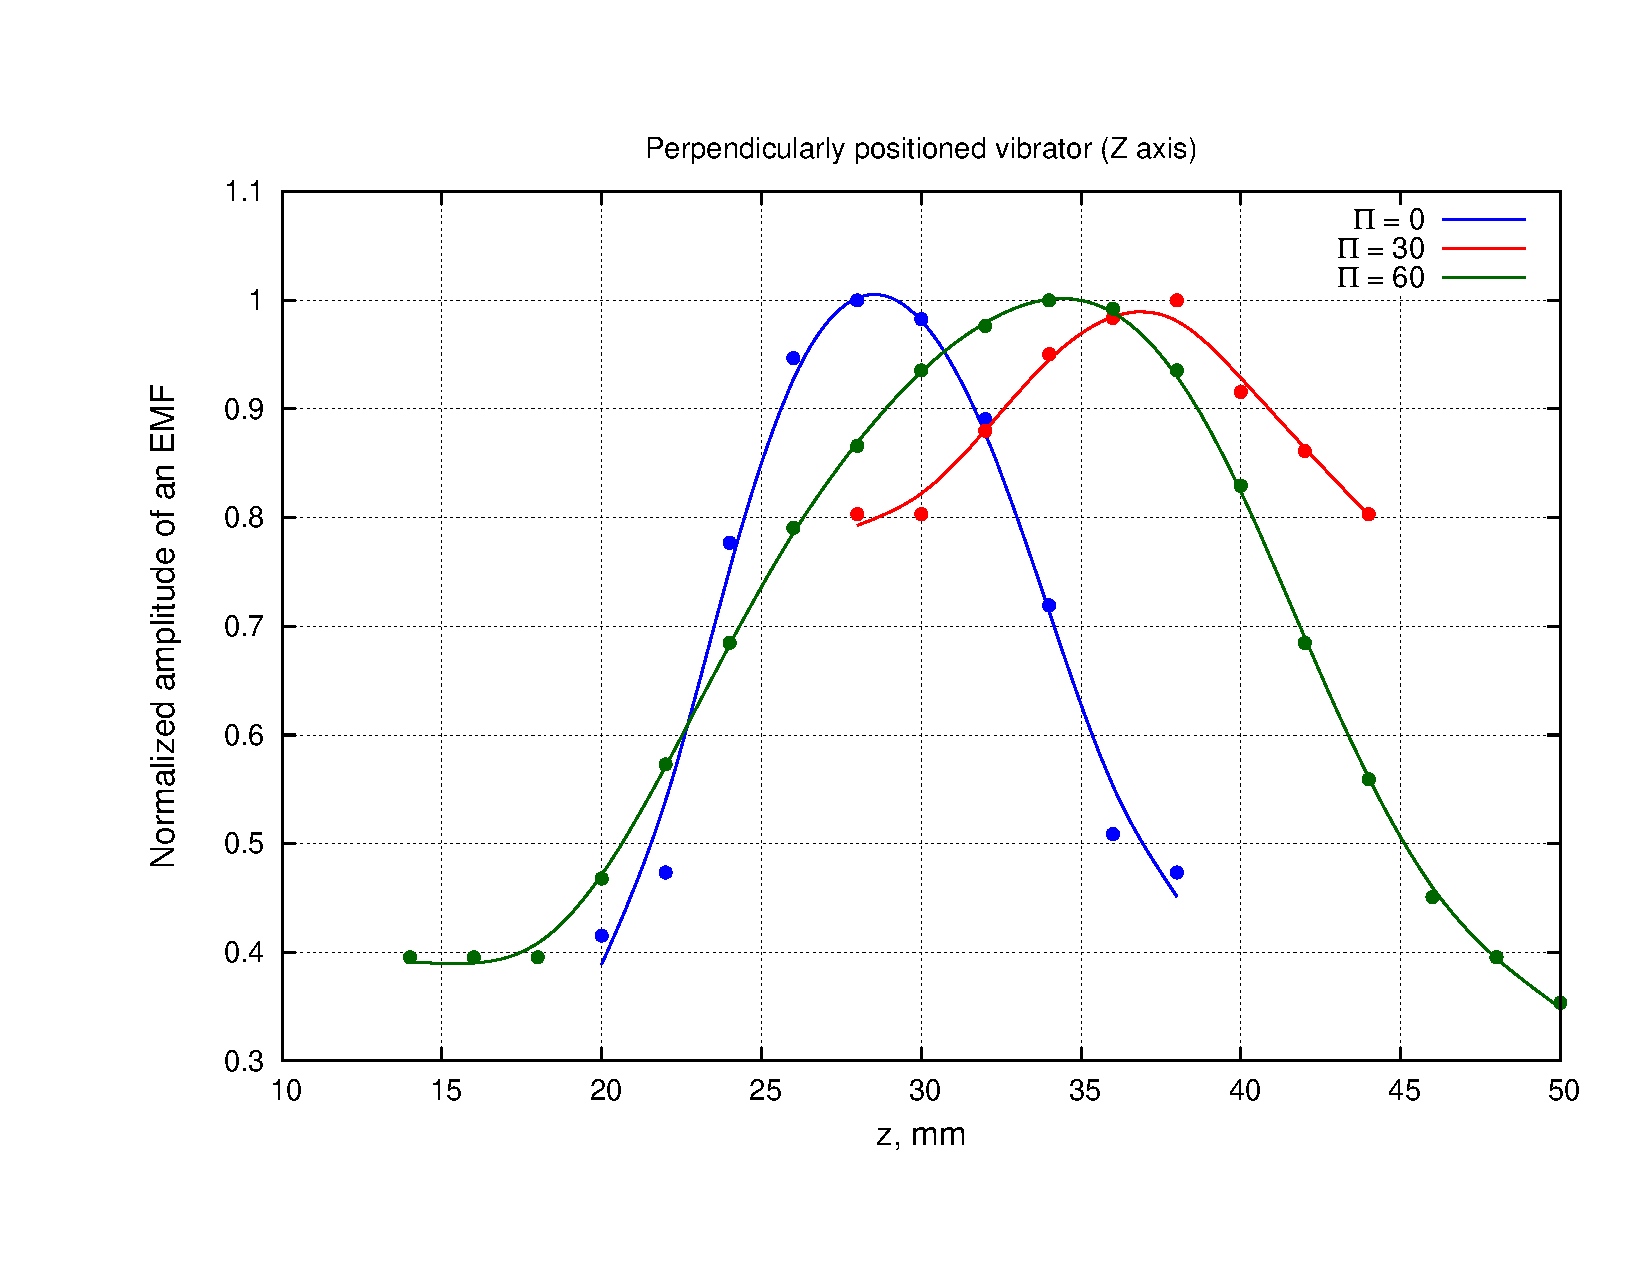
\includegraphics[width=\textwidth]{plot1.pdf}
    \end{center}
    \vspace {-20 pt}
    \caption{График зависимости составляющих $|\overline{E}_{\Sigma_y}(z)|$}
    \label{fig:plot1}
\end{figure}

\begin{figure}[hb!]
    \begin{center}
        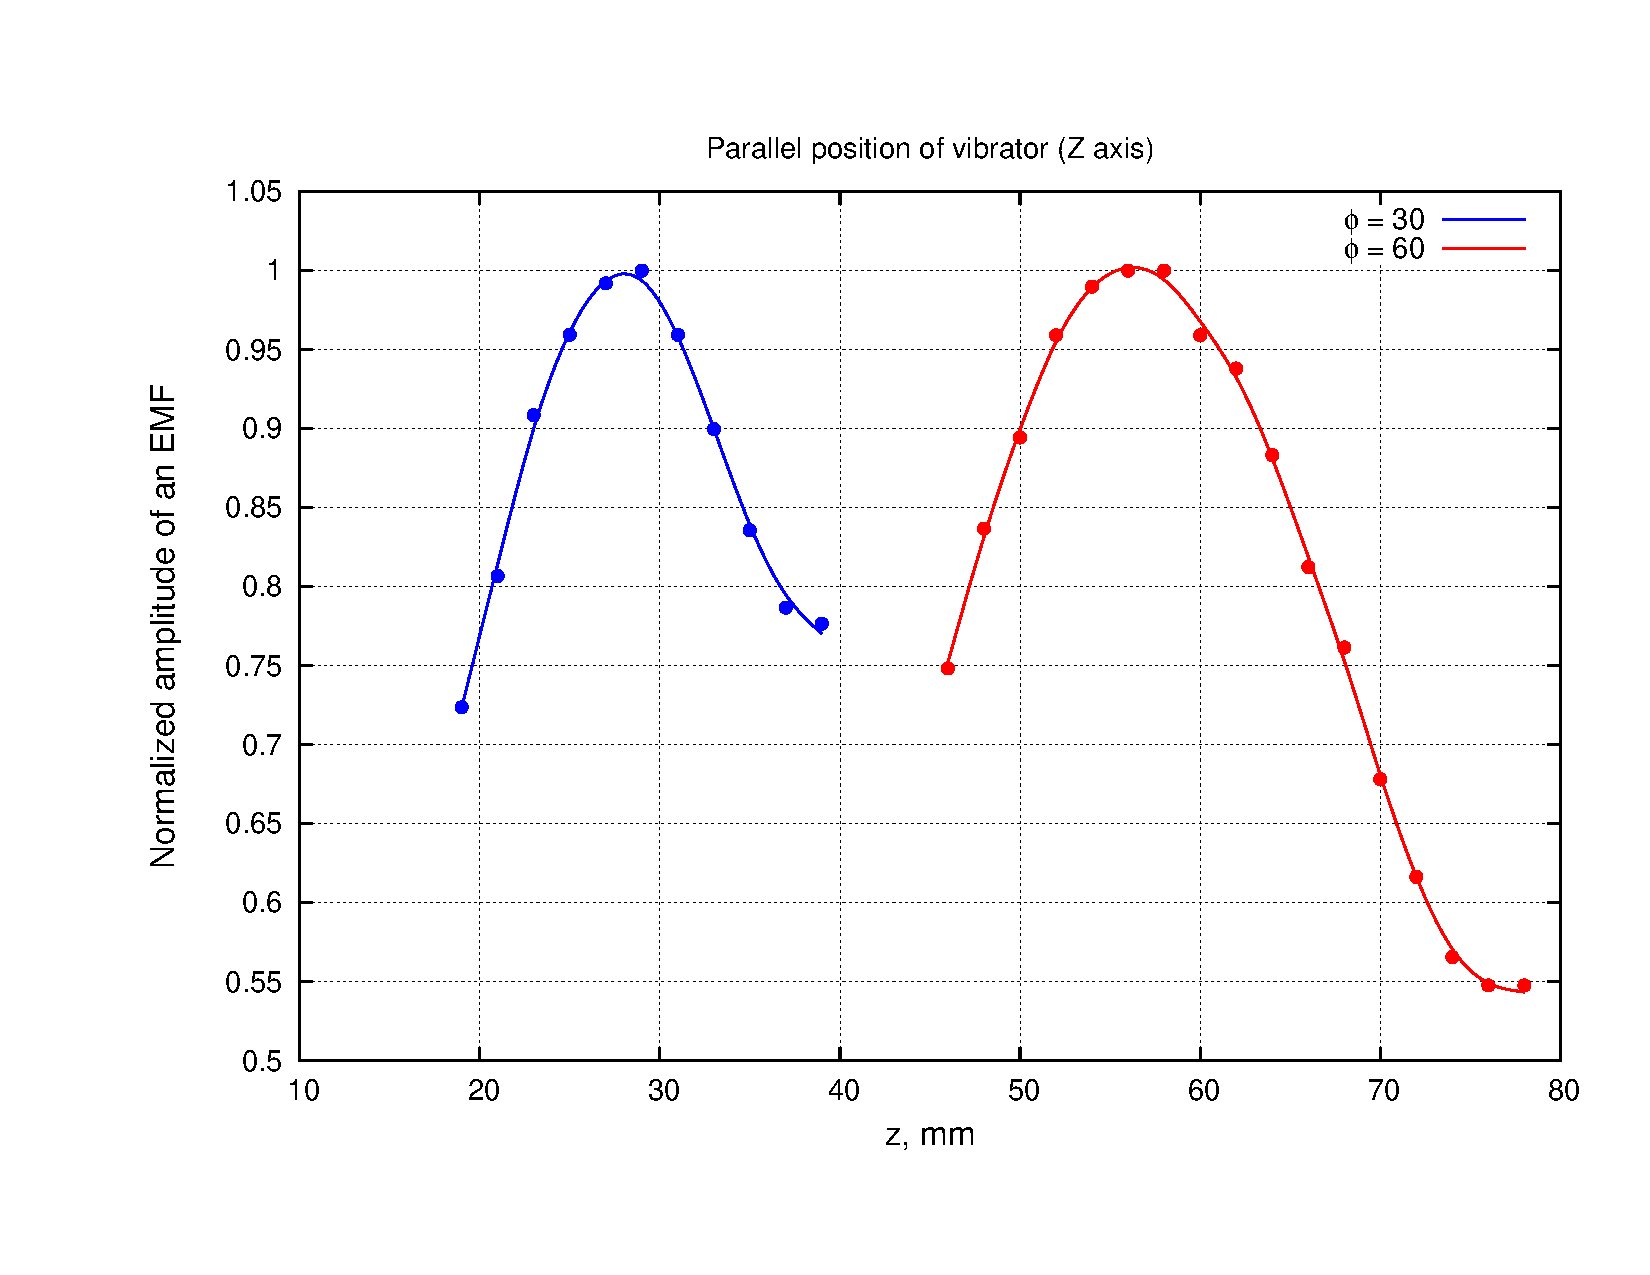
\includegraphics[width=\textwidth]{plot2.pdf}
    \end{center}
    \caption{График зависимости составляющих $|\overline{E}_{\Sigma_z}(z)|$}
    \label{fig:plot2}
\end{figure}

\begin{figure}[hb!]
    \begin{center}
        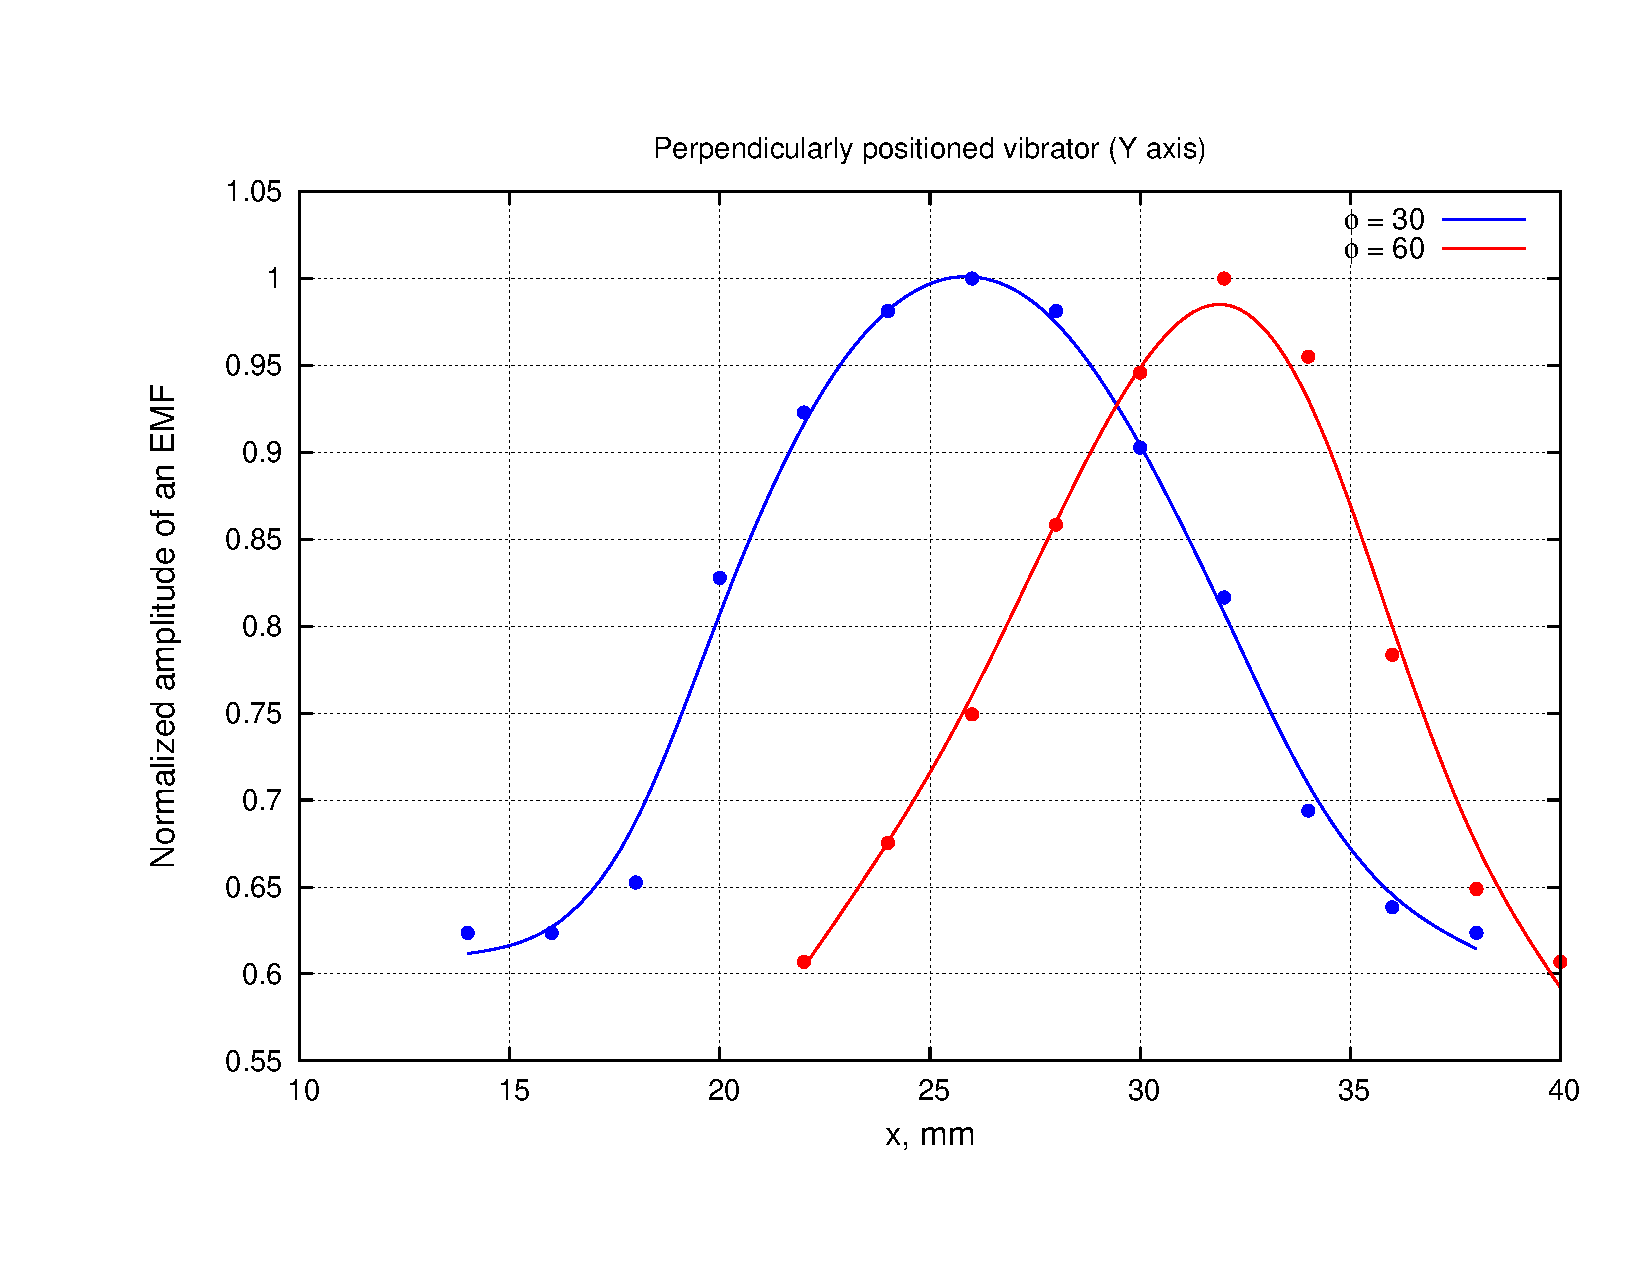
\includegraphics[width=\textwidth]{plot3.pdf}
    \end{center}
    \vspace {-20 pt}
    \caption{График зависимости составляющих $|\overline{E}_{\Sigma_y}(y)|$}
    \label{fig:plot3}
\end{figure}

\begin{figure}[h!]
    \begin{center}
        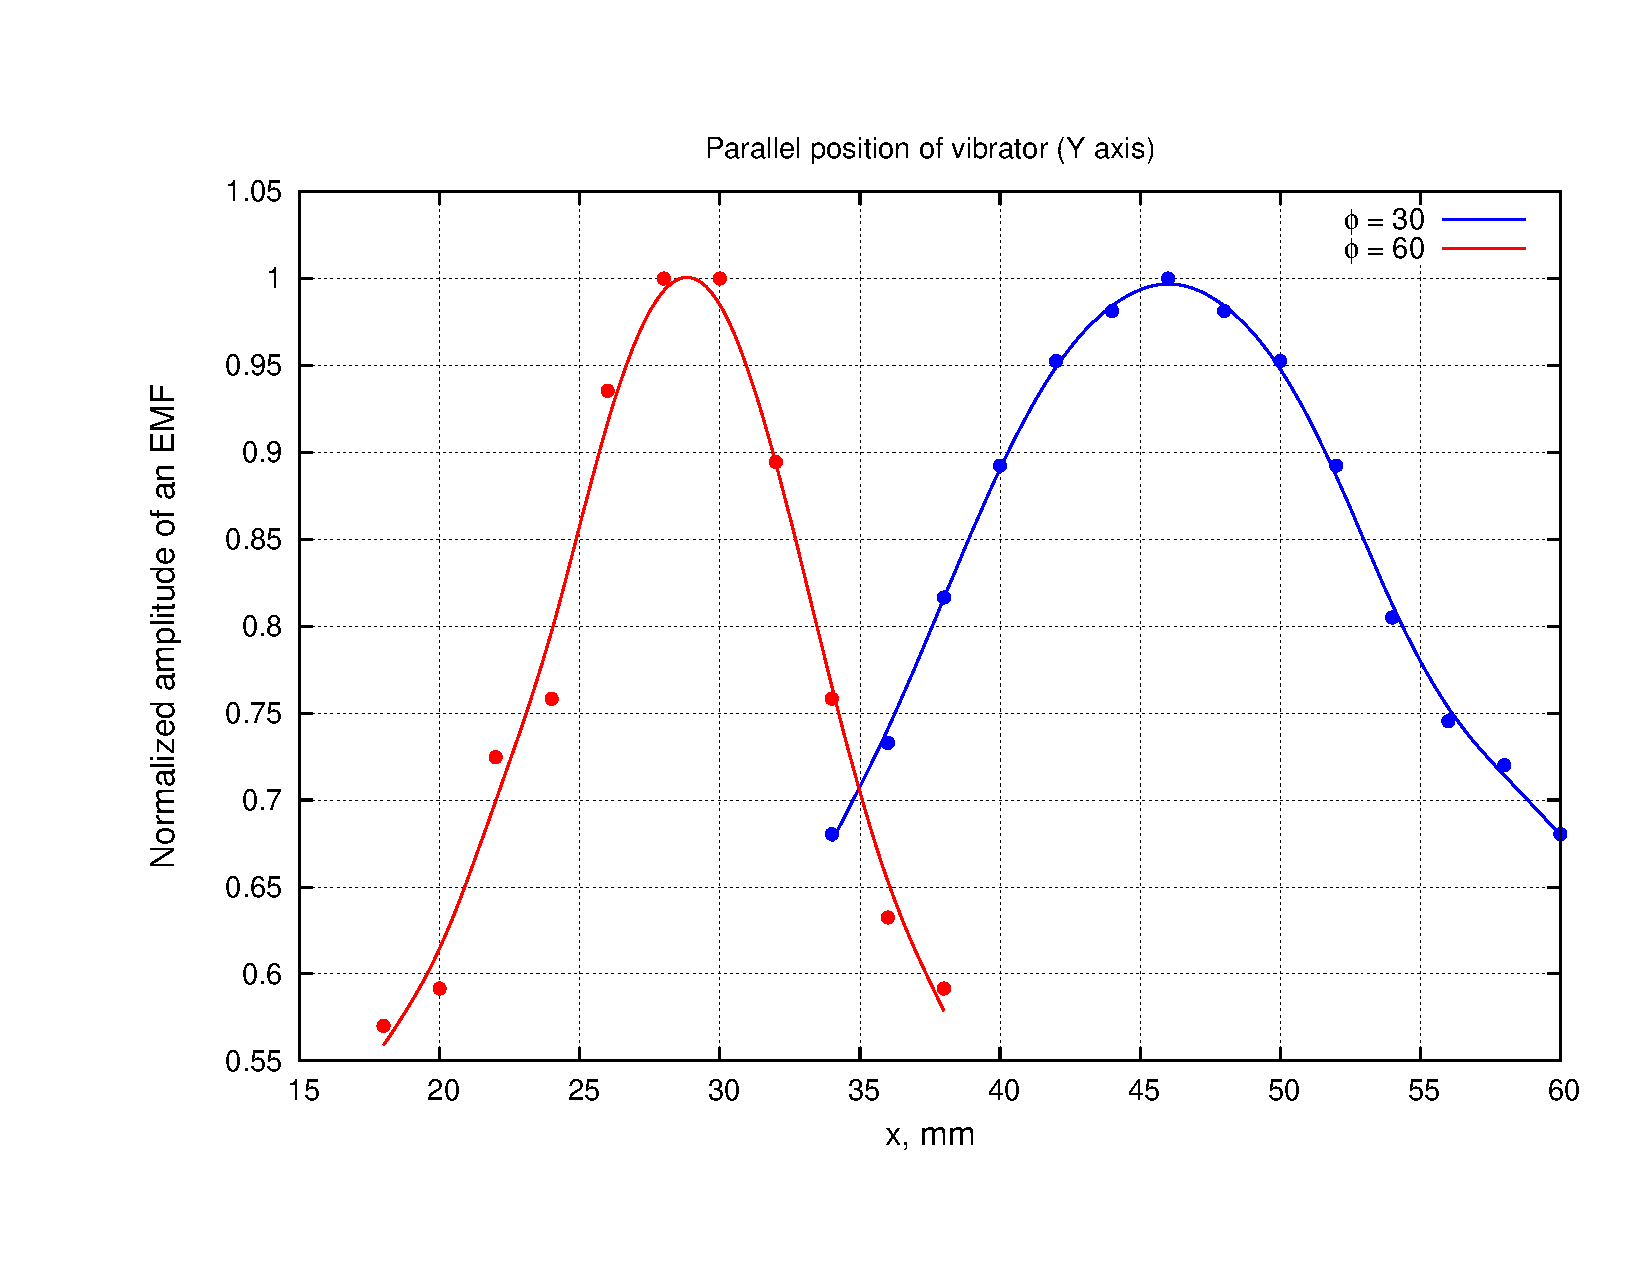
\includegraphics[width=\textwidth]{plot4.pdf}
    \end{center}
    \vspace {-20 pt}
    \caption{График зависимости составляющих $|\overline{E}_{\Sigma_z}(y)|$}
    \label{fig:plot4}
\end{figure}

\vspace{10pt}
\section{Выводы}
Проведено полное исследование структуры электромагнитного поля над плоской проводящей
поверхностью. Форма полученных экспериментальных кривых подтверждается
теоретическими выкладками. При росте угла отклонения источника электромагнитных
волн наблюдается сглаживание
экспериментальной кривой при сохранении её основных свойств по оси ординат. Этот факт может
объясняться ростом рассеяния и отражения волны от неучтённых поверхностей лабораторного
помещения.
\end{document}
